\subsection{\acs{NIST} Special Publication 800-61}
This subsection gives an introduction to the guidelines \acs{NIST} SP 800-61 and the content is, unless specified otherwise, derived from \cite{nist800-61}. This publication aims to  assist organizations in mitigating risks from computer security incidents by providing guidelines on how to respond to incidents effectively and efficiently. 

The security-related threat level is continuously changing and new types of security-related incidents emerge frequently. Preventive actions are not sufficient in order to be able to handle this and an incident response capability is therefore necessary. Even though incident prevention is not sufficient, it is an important complement to incident response. The existence of an incident response capability in an organization can assist them in rapidly detecting incidents, minimizing loss and destruction, mitigating the weaknesses that were exploited and restoring computing services. It is important to note that incident response requires a substantial amount of planning and resources. Some of the most important parts of incident response are the existence of guidelines related to communication and related to prioritizing incidents and the use of a lessons learned process to gain value from incidents.

One of the first considerations for a \ac{CSIRC} should be to agree on a definition of the term incident. This guidelines' definitions of event and incidents are included in section \ref{sec:Definitions} of this report. An organization should have an incident response policy, an incident response plan and incident response procedures, all of which should be tailored to the specific organization's needs. The policy usually includes elements such as prioritization or severity ratings of incidents, a definition of computer security incidents and reporting and contact forms. The plan usually includes an organizational approach to incident response, how the incident response team will communicate with the rest of the organization and with other organizations and metrics for measuring the incident response capability. Procedures should be based on the incident response policy and plan and \acp{SOP} are a delineation of the specific technical processes, techniques, checklists and forms used by the incident response team. An organization should establish procedures regarding communication with various outside parties, like media, law enforcement, other incident response teams, software vendors and \acp{ISP}. It is common to have \acp{PoC} for the various outside parties. 

Organizations should have an incident response team available to handle incidents. The number of people responding depends on the magnitude of the incident. Large organizations can choose to have several incident response team, e.g. one team per division. The teams can consist of employees or be partially or fully outsourced. The team members can be full-time or part-time depending on funding, staffing and incident response need.  %More about teams? Perhaps not necessary?
An incident response team usually perform intrusion detection, advisory distribution and education and awareness in addition to incident response.

\acs{NIST} SP 800-61 describes the four phases of incident response; preparation, detection and analysis, containment, eradication and recovery and post-incident activity. The phases and the relationship between them is illustrated in figure \ref{fig:NISTIncidentResponse}.

\begin{figure}[ht]
%\hspace*{-0.4cm}
\begin{center}
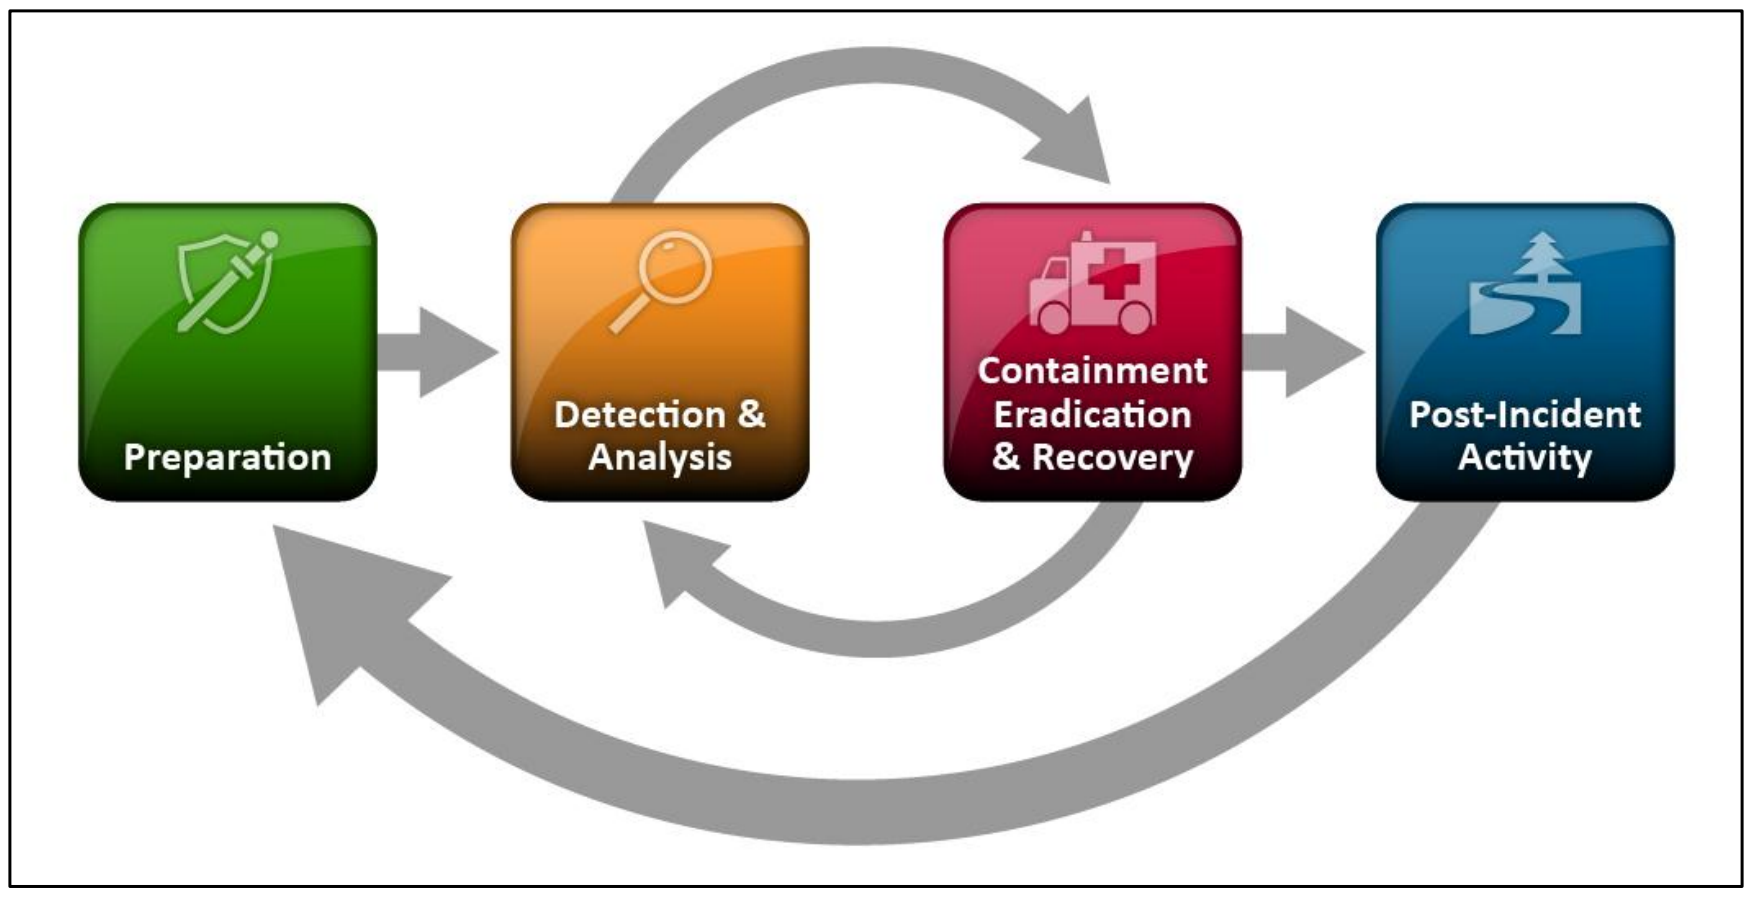
\includegraphics[scale=0.27]{NISTIncidentResponseCycle.png}
\caption[The Incident Response Life Cycle]{The Incident Response Life Cycle \cite{nist800-61}}
\label{fig:NISTIncidentResponse}
\end{center}
\end{figure}

\paragraph{Preparation} 
This phase includes establishing an incident response capability as well as preventing incidents. The latter is not typically a part of the incident response team's tasks, but it is fundamental to the success of the organization's incident response. If a large number of incidents occur, it may overwhelm the incident response team. To prepare for incidents the incident handlers should have tools and resources like contact information, incident reporting mechanisms, issue tracking system, digital forensic workstations\footnote{A digital forensic workstation is specially designed for acquiring and analysing data. It usually contains a set of removable hard drives that can be used for evidence storage.} and digital forensic software. It is common to create a portable \emph{jump kit} containing materials that may be needed during incident response.

\paragraph{Detection and Analysis}
Organizations should prepare to handle any type of incident and to handle common incident types. A classification of incidents can be used as a basis for incident handling. The guidelines provides a list of example categories that contains web, email, improper usage and loss or theft of equipment. This guidelines focuses on handling of any type of incident and not specific categories. A challenge related to incident handling is to actually detect the incident and determine the potential impact the incident may have. The actual detection may be the hardest part of incident handling. The guidelines defines two types of signs of incidents; precursors and indicators, with indicators being the most common. These are defined in the following way: "A \emph{precursor} is a sign that an incident may occur in the future. An \emph{indicator} is a sign that an incident may have occurred or may be occurring now." Common sources for precursors and indicators are \acp{IDPS}, antivirus and antispam software, third-party monitoring services, logs, information on new vulnerabilities and exploits and people. 

A challenging part of this phase is the analysis, i.e. to determine which indicators and precursors are legitimate, if they are really related to an incident and what has actually happened. When the team believes an incident to have occurred they should try to determine the scope. All steps taken should be documented and timestamped. It is important to note that any such documentation can be used in court. The incident response team should maintain a database containing information about incidents, such as status, indicators, related incidents and actions taken by the incident handlers. It is important to prioritize incidents and handle them accordingly. Factors that can be used as a basis for prioritization include the functional impact of the incident, the information impact of the incident and recovery from the incident. When the prioritization is performed the incident response team should notify the appropriate people. It is important to have procedures regarding who these people should be.

\paragraph{Containment, Eradication and Recovery}
Containment is obviously an important part of incident handling. The existence of strategies and procedures for containment is helpful. These strategies and procedures are different for different types of incidents. 

\paragraph{Post-Incident Activity}


